\documentclass[12pt, a4paper, addpoints]{exam} % addpoints: 允许在每题后指定分数

% 1. 中文字体和页面设置
\usepackage{xeCJK}
%\usepackage{exam}
\setCJKmainfont{Source Han Serif SC} % 使用思源宋体,请确保系统已安装
\usepackage[inner=2cm, outer=2cm, top=2cm, bottom=2cm]{geometry}
\usepackage{amsmath, amssymb} % 数学公式和符号
\usepackage{graphicx}
\usepackage{setspace} % 用于设置行距

% --- 将分值单位改成“分”,并显示为“(10分)” ---
\pointname{分}                % “10分”;若想有空格就写 { 分}
\marginpointname{分}          % 右/左边距里的分值单位(若你用 \pointsinmargin)
\bonuspointname{分}           % 赠分题(如果会用到)
\pointformat{(\thepoints)}    % 题目前显示成 “(10分)”
% -----------------------------------------------


% 2. 自定义作业信息
\def\TitleName{初三数学课后作业 (隐圆与二次函数)}
\def\TeacherName{}
\def\chinesedate{\the\year 年\the\month 月\the\day 日}
\def\ClassName{}

% 3. 页眉和页脚设置
\pagestyle{headandfoot} % 启用 exam 宏包的页眉页脚

% 页眉内容(\small 是为了让字体小一点)
\lhead{\small \TitleName}               % 左页眉:作业名称
\chead{\small 授课教师:\TeacherName}    % 中页眉:教师
%\rhead{\small 成绩:\ClassName}         % 右页眉:班级
\footer{}{\thepage}{}                   % 页脚:只在中间显示页码

% 页眉下方横线和间距
\renewcommand{\headrule}{%
  \hrule height 0.4pt
  \vspace{6pt} % 页眉和正文间距
}


\begin{document}

% 顶部信息和总分
%\noindent\textbf{姓名:\qquad\qquad\qquad\qquad 成绩:\rule{3cm}{0.4pt}}
\vspace{10pt}


%=========================== 题目区 ===========================

\begingroup\setstretch{1.35} % 设置行距为1.35倍行距

\begin{questions}

% --- 题目开始 ---

% 显示为 (10分)
\question[10] 如图,在四边形 $ABCD$ 中,$\angle{ABC}=\angle{D}=90^{o}$,连接 $AC$,点F为 $CD$ 边上一点,
连接 $BE$ 交 $AC$ 于点E,$AB=AE$,$\angle{FGC}+\angle{FBG}=90^{o}$,$\angle{BFG}+2\angle{GFC}=180^{o}$,
若 $AD=\frac{7\sqrt{2}}{2}$,$BG=4$,则$CG$的长为 \rule{3cm}{0.4pt}.

\ \ 
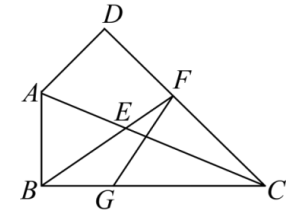
\includegraphics[scale=1]{2222.png}
\vspace{6cm}




% 总分显示为 (15分)
\question[15] 如图,二次函数 $y=-x^2+2mx+2m+1 $ (m是常数,且 $m>0$)的图象与x轴交于A,B两点(点A在点B的
左侧),与y轴交于点C,顶点为D.其对称轴与线段 $BC$ 交于点E,与x轴交于点F.连接 $AC$.若 $\angle{BEF}=2\angle{ACO}$ ,
则m的值是多少?

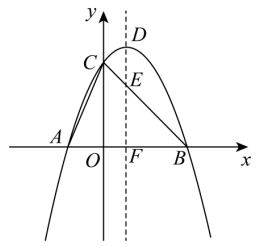
\includegraphics[scale=1]{1111.png}
\vspace{6cm}


\end{questions}
\endgroup
\end{document}